\documentclass[12pt]{iopart}

% \usepackage{citesort}
\usepackage[square,sort&compress]{natbib}
\usepackage{amsmath} % For maths
\usepackage{graphicx}	% For graphics
\usepackage{enumerate}  % For numbered lists
\usepackage{hyperref}	% For hyperreferences
\usepackage{booktabs}   % For professional-looking tables
\hypersetup{colorlinks=false}
\hfuzz=4pt

%==============================================================================
% From iopart
\newcommand{\BibTeX}{Bib\TeX}
\newcommand{\REVTeX}{REV\TeX}

% \bibliographystyle{iopart-num}

%==============================================================================
% Macros specific to this paper.
\newcommand{\hl}[1]{\textnormal{\textbf{#1}}} % highlight, esp. a definition
\newcommand{\nside}{N_{\text{side}}}
\newcommand{\IDparent}{ID_{\text{common~parent}}}
\newcommand{\IDchild}{ID_{\text{relative~child}}}
% \newcommand{\id}{ID} % \DeclareMathOperator{\id}{ID}
% \newcommand{\rid}{rowID} % \DeclareMathOperator{\rid}{rowID}
% \newcommand{\cid}{colID} % \DeclareMathOperator{\cid}{colID}

\sloppy 

%==============================================================================
% Front matter.
\begin{document}
% \nocite{*}
\pagestyle{empty}

\title{The rHEALPix Discrete Global Grid System}

\author{R~G~Gibb}

\address{Informatics Team Leader, Landcare Research, Private~Bag~11052, Palmerston~North~4442, New~Zealand}

\eads{gibbr@landcareresearch.co.nz}

\begin{abstract}
In light of the new standard for Discrete Global Grid Systems (DGGS) currently being proposed by the Open Geospatial Consortium (OGC), we revisit our earlier work on defining the rHEALPix DGGS. This paper briefly restates the definition of the rHEALPix DGGS and shows  how the cell geometries, and schema for cell identifiers are both compliant with the standard. We then show that the fundamental topological operators, required by the standard can be implemented directly by manipulation of the cell identifiers without reference to or knowledge of traditional coordinates.
\end{abstract}

%-----------------------------------------------------------------------------
\section{Introduction}\label{sec:introduction}
Early work characterising discrete global grid systems (DGGS) \citep{KSWS1999, SWK2003} focused on identifying a broad set of ideal geometric properties for DGGS and establishing measures to assess the deviation from the ideal across the globe. Using these measures different DGGS geometries could be compared and DGGS identified to meet the geometric needs of particular applications. In the decade since this early work practitioners realised that geometry alone wasn't sufficient for defining a useful DGGS, and that for instance a cell addressing scheme was also needed \citep{GiRa2013}.  The OGC DGGS Standards Working Group \citep{PGP2014} has gone further and now proposes that standard DGGS must ``define a hierarchical tessellation of equal area cells that both partition the entire Earth at multiple levels of granularity and provide a global spatial reference frame.'' but also provide ``encoding methods to: address each cell; assign quantized data to cells; and perform algebraic operations on the cells and the data assigned to them.''

The new definition for DGGS contrasts with earlier usage in two important ways. 
\begin{enumerate}[(i)] 
    \item Early work \citep{Good1994, KSWS1999, SWK2003} focused on defining a set of 14 geometric criteria---the 'Goodchild Criteria'---for grids that should be taken into account in designing a good DGGS. Since it is mathematically impossible \citep{KSWS1999} to completely fulfill all the 'Goodchild Criteria' the OGC standard identifies an essential subset of geometric criteria that can be simultaneously satisfied by a number of different approaches to DGGS design.
    \item While early work focused primarily on geometry, the OGC standard recognises the emerging demands of spatial big-data analysis, linked spatial data and DGGS interoperability need a new digital spatial reference system for the whole-earth. Despite pre-dating the era of the internet and bigdata,  Goodchild also foresaw the need for an addressing system and efficient algorithms supporting common grid operations in his criteria \citep{Good1994}, though he didnt stipulate what those operations should be. The OGC standard therefore identifies a specific set of fundamental operations that the spatial reference system's addressing scheme should support. 
\end{enumerate}

The HEALPix DGGS introduced in \citep{GHBW2005} to support  cosmic microwave background radiation studies, defines a family of related DGGS each with the following features:
\begin{enumerate}[(i)] 
    \item Cells that are hierarchical, congruent, aligned for odd values of an integer parameter $\nside$, and constant aperture, which makes it easy to implement with efficient data structures, and easy to establish cell addressing schemes.
    \item At every resolution their grid cells have equal areas, which provide equal probabilities for statistical analyses, and ensure environmental properties assigned to each cell have equivalent meaning. 
    \item At every resolution their grid cells cover the entire globe, so that area is preserved throughout the hierarchy, and every cell has a nucleus that can be used as a reference point.
    \item At each resolution their $k$ nuclei lie on only $\Theta(\sqrt{k})$ parallels of latitude, which makes computing spherical harmonics fast.
    \item Their planar projections have low average angular and linear distortion.
\end{enumerate}
In our original paper \citep{GiRa2013}, while preserving features (i)--(v), we extended the HEALPix DGGS from a purely spherical solution suitable for astronomical use to:
\begin{enumerate}[(i)] 
    \item[(vi)] Ellipsoids of revolution such as the WGS84 ellipsoid, which is more suitable for terrestrial use.
\end{enumerate}

Finally we elaborated on the work of \citep[Section 3.1]{CaRo2007}, by rearranging the underlying HEALPix map projection into what we called the rHEALPix map projection and built a DGGS for ellipsoids of revolution based upon it, which we called the rHEALPix DGGS.
The rHEALPix DGGS also has features (i)--(vi) and additionally:
\begin{enumerate}[(i)]
    \item[(vii)] Its base polyhedron---the cube---is a regular polyhedron. 
    \item[(viii)] Its planar projection consists of horizontal-vertical aligned nested square grids, which are widely used in remote sensing and in environmental modelling.
\end{enumerate}

Features (i)--(iii) and (vii) are sufficient to meet the cell geometry requirements of the proposed OGC DGGS standard, and features (i), (iv) and (viii) significantly assist in designing an indexing system with efficient conversion to and from latitude longitude coordinates, which we describe below.

%-----------------------------------------------------------------------------
\section{Defining the rHEALPix DGGS}\label{sec:definition}

The rHEALPix DGGS can be thought of as a mapping of an ellipsoid of revolution onto a regular polyhedron, namely a cube, see figure~\ref{fig:cube}, followed by a symmetric hierarchical partitioning of the polyhedral faces along with a choice of nuclei, followed by the inverse mapping of the result back onto the ellipsoid, see figure~\ref{fig:grids}. It is therefore an example of a cubic geodesic DGGS \citep{SWK2003}. The rHEALPix DGGS and its associated mathematics have been fully described by us  in \citep{GiRa2013}. 

To support transfer of data into and out of both rHEALPix and HEALPix we have implemented the mathematics for both projections in the PROJ.4 cartographic library (from release 4.8), allowing us to use standard raster manipulation tools. Using the PROJ.4 library as a link to traditional GIS libraries provides a fundamental building block for satisfying the proposed OGC DGGS Standard's requirement for provision of operations for assigning data to and retrieving data from cells.

\begin{figure}[!htb] 
\centering
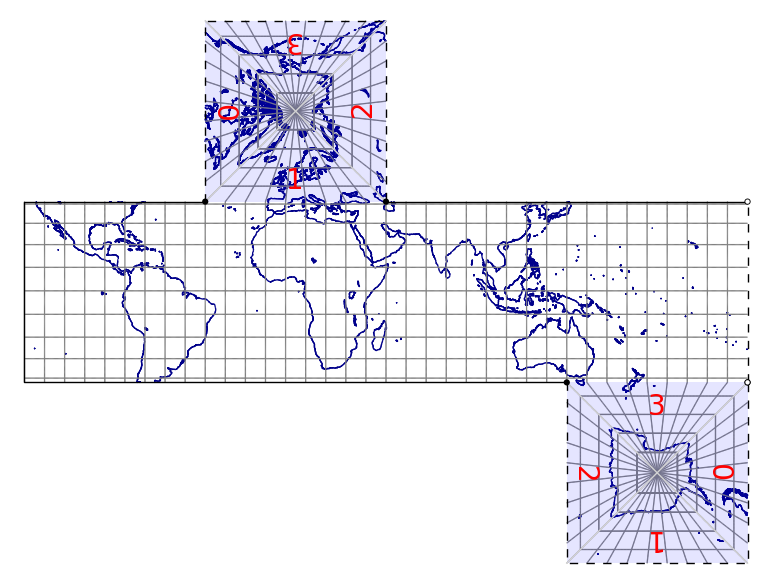
\includegraphics[width=\textwidth]{fig-projections_rhealpix_13_50deg.png}
\caption{The (1,3)-rHEALPix projection of the WGS84 ellipsoid with a $10^\circ$ graticule.
To illustrate some (r)HEALPix projection options, the prime meridian has been shifted to $50^\circ$ east longitude to move all cube's corners into water, Arctic polar triangle boundary cuts to less densely populated regions, and rearranged polar triangles to the (1,3) position to optimise Europe and New Zealand views.}
\label{fig:cube}
\end{figure}

\begin{figure}[!htb]
\centering
$G_0$ 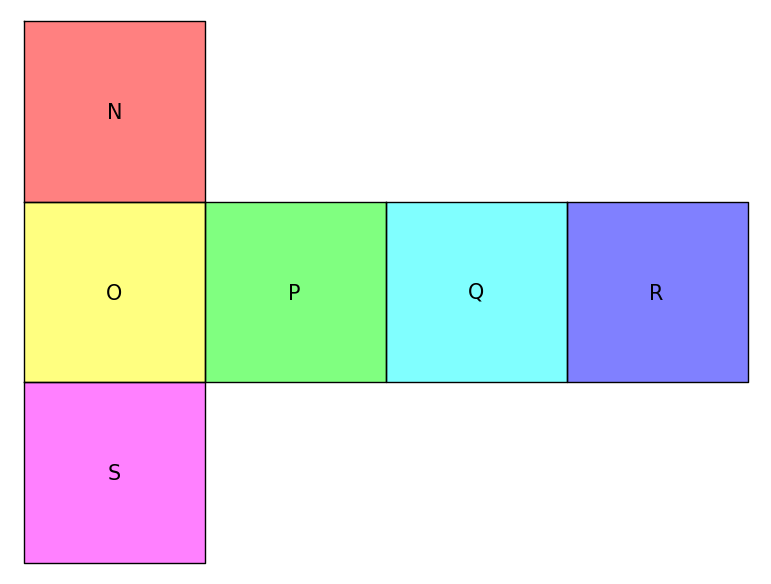
\includegraphics[height=55mm]{fig-grids_grid0_00.png} \qquad
$G'_0$ 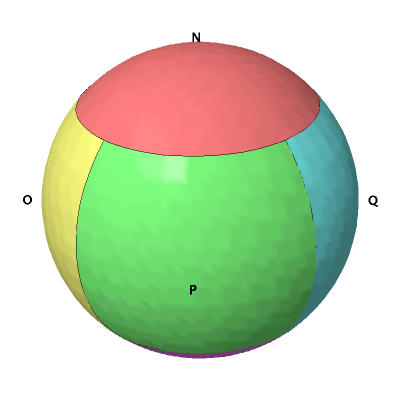
\includegraphics[height=55mm]{fig-grids_grid0_00_ellipsoid.png} \\
$G_1$ 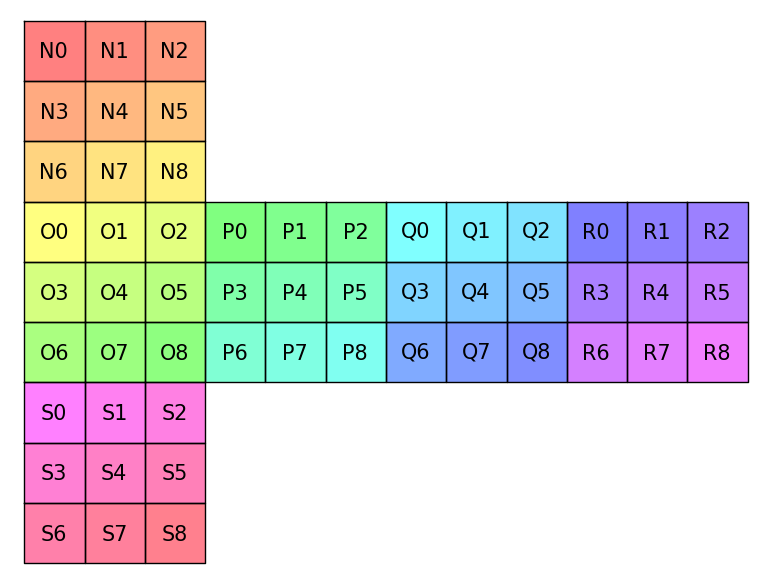
\includegraphics[height=55mm]{fig-grids_grid1_00.png} \qquad
$G'_1$ 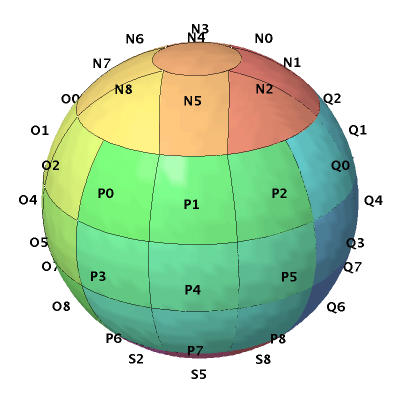
\includegraphics[height=55mm]{fig-grids_grid1_00_ellipsoid.png} \\
\caption{The first two planar and ellipsoidal grids for the (0, 0)-rHEALPix map projection with $\nside = 3$ and cells labelled with their IDs.}
\label{fig:grids}
\end{figure}

% To extend the rHEALPix DGGS from a sphere to the ellipsoid while preserving features (i)--(v) we (a) map the WGS84 ellipsoid onto its authalic sphere preserving area; (b) map the authalic sphere onto the plane with the rHEALPix projection; (c) define the horizontal-vertical aligned rHEALPix square grid system; (d) map this grid system back to the ellipsoid by applying inverse projections.
% This process preserves features (i)--(v) of the rHEALPix DGGS, because the map in step (a) preserves local areas, sends meridians to meridians, parallels to parallels, and has low average distortion.
% For HEALPix and rHEALPix projections mathematics, see \citep[Appendix A and B]{GiRa2013}.

% More specifically, for step (b) map the authalic sphere to the plane via the $(n, s)$-rHEALPix projection for integers $0 \le n, s \le 3$; see figure~\ref{fig:projections}.
% The $(n, s)$-rHEALPix and HEALPix projections are equi-areal with area scaling factor $3\pi/8$.

% For step (c), recursively construct a sequence $G_0, G_1, G_2, \ldots$ of nested grids on the planar projection with $G_0$ the set of 6 squares of our cube.
% Choose an integer $\nside \ge 2$, and for each integer $i \ge 0$ let $G_{i+1}$ be the grid obtained by refining each square of grid $G_i$ into $\nside \times \nside$ isomorphic sub-squares.
% Then each grid $G_i$ comprises $6 \cdot \nside^{2i}$ isomorphic square cells, each having side length $R_q (\pi/2) \nside^{-i}$ and area $R_q^2 (\pi^2/4) \nside^{-2i}$.
% Define the nucleus of each cell to be its centroid.
% We refer to each planar grid $G_i$ as the \hl{$(n, s)$-rHEALPix planar grid of resolution $i$}, and the nested sequence $G:= (G_0, G_1, G_2, \ldots)$ of planar grids the \hl{$(n, s)$-rHEALPix planar grid hierarchy}; see $G_0, G_1$ figure~\ref{fig:grids} .
% Strictly, $G$ is not a DGGS, since each of its grids partition a planar projection of the ellipsoid rather than the ellipsoid itself.

% For step (d), map each planar grid $G_i$ and its nuclei set back to the ellipsoid via the inverse $(n, s)$-rHEALPix projection, call the resulting ellipsoidal grid $G'_i$ the \hl{$(n, s)$-rHEALPix ellipsoidal grid of resolution $i$}, and call the nested sequence $G':= (G_0', G_1', G_2', \ldots)$ of ellipsoidal grids the \hl{$(n, s)$-rHEALPix ellipsoidal grid hierarchy}; see $G_0', G_1'$ figure~\ref{fig:grids}.
% This hierarchy is the \hl{$(n, s)$-rHEALPix DGGS}.
% All resolution $i$ cells have equal area of $R_q^2 (\pi^2/4) \nside^{-2i} /(3\pi/8) = R_q^2 (2\pi/3) \nside^{-2i}$, because $(n, s)$-rHEALPix map projection is equi-areal with area scaling factor $3\pi/8$.
% From figure~\ref{fig:grids} each grid $G'_i$ comprises $6 \cdot \nside^{2i}$ cells of four different shapes which we call quad, skew quad, dart and cap cells. All cells on equatorial faces (O, P, Q, R) are \hl{quad cell}s, e.g. P0, P1, P2 etc; cells containing a pole are \hl{cap cell}s e.g N4; cells on diagonals of polar faces (N, S) are \hl{dart cell}s e.g. N8; and remaining polar face cells are \hl{sqew quad cells} e.g. N5. Every cell's shape can be determined directly from it's \hl{ID}. 

From here forward we focuses on a (0,0)-rHEALPix DGGS with $\nside = 3$, producing aligned hierarchies with the smallest change of area between resolutions. Table~\ref{tab:cell_stats} provides cell dimensions for a selection of resolutions using this DGGS. 

\begin{table}[!htb]
\center{\begin{tabular}{cccc}
\toprule
Resolution & Cell area (m$^2$) & Nominal cell edge & Number of cells \\
\midrule
 0  &  85.11E+12  &  9,225 km  &        6    \\
1  &  9.456E+12  &   3,075 km  &       54 \\
2  &  1.051E+12  &    1,025 km  &  486 \\
% 3  &  1.2E+11  &  3.4E+05  &  4.4E+03 \\
% 4  &  1.3E+10  &  1.1E+05  &  3.9E+04 \\
 % .. \\
% 5  &  1441.3E+06  &  3.8E+04  &  354,294 \\
% 6  &  160.14E+06  &  12,654  &  3,188,646 \\
% 7  &  17.793E+06  &  4,218  &  28.7E+06 \\
% 8  &    1.977E+06  &  1,406  &  258.3E+06 \\
% 9  &  2.2E+05  &  4.7E+02  &  2.3E+09 \\
% 10  &  2.4E+04  &  1.6E+02  &  2.1E+10 \\
 .. \\
11  &  2,712  &      54 m &    188.3E+09 \\
12  &     301  &      18 m &  1,694.6E+09 \\
13  &    33.5  &         6 m &  15,251E+09 \\
14  &    3.72  &         2 m &  137.26E+12 \\
% 15  &     0.41  &     0.64  &  1.2E+15 \\
\bottomrule \\
\end{tabular}}
\caption{Approximate cell area, nominal cell edge length, and number of cells for a selection of grid resolutions of the $\nside = 3$ WGS84 ellipsoidal rHEALPix grid hierarchy.}
\label{tab:cell_stats}
\end{table}

% Besides being hierarchical and recursive, the hierarchies $G$ and $G'$ are both \hl{congruent}, that is, each resolution $i$ cell is a union of resolution $i + 1$ cells; when $\nside$ is odd the hierarchies $G$ and $G'$ are both \hl{aligned}, that is, each resolution $i$ cell nucleus is the nucleus of a resolution $i + 1$ cell; the hierarchies $G$ and $G'$ both have a \hl{constant aperture} of $\nside^2$, that is, each resolution $i$ cell has $\nside^2$ times the area of its resolution $i + 1$ child cells.

%-----------------------------------------------------------------------------
\section{Constructing cell identifiers}\label{sec:cellid}
For reference we assign unique names to the cells of the planar hierarchy $G$ that are shared with the corresponding cells of the ellipsoidal hierarchy $G'$.
These names echo the tree structure of the hierarchies and are defined as follows.

Let $\Gamma$ be the set of all strings beginning with one of the letters $N, O, \ldots, S$ and followed by zero or more of the integers $0, 1, \ldots, 3^2 - 1$, so that $\Gamma$ forms a regular language $(N | O | \cdots | S)(0 | 1 | \cdots | 8)^*$. The identifier (ID) of a cell $c$ from $G$, denoted $c$, is the string in $\Gamma$ defined recursively as follows.
Assign the cells of $G_0$ the IDs $N, O, P, Q, R, S$ from top to bottom and left to right.
In particular, cell $N$ contains the projection of the north pole and cell $S$ contains the projection of the south pole.
For each resolution $i$ cell with ID $s$ assign its $9$ resolution $i + 1$ child cells the IDs $s0, s 1, \ldots, s 8$ following the path of a $Z$ space filling curve from top to bottom and left to right; see figure~\ref{fig:children}(a). 

\begin{figure}[!htb]
\label{fig:children}
  \center{(a) 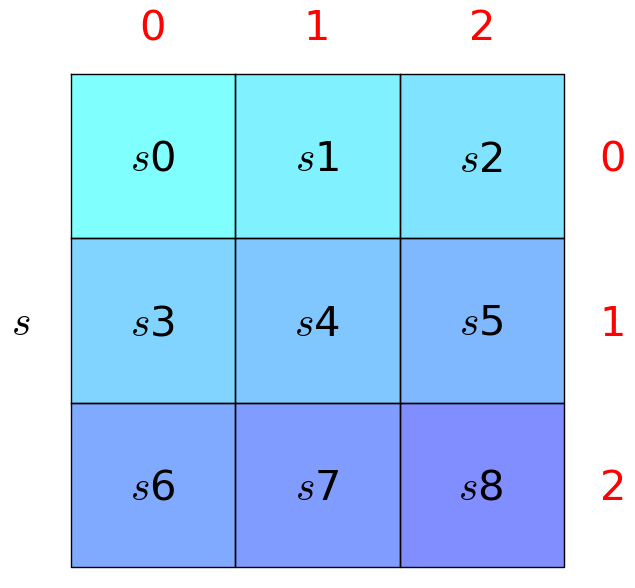
\includegraphics[scale=0.37]{fig-children_children.png} 
  \qquad (b) 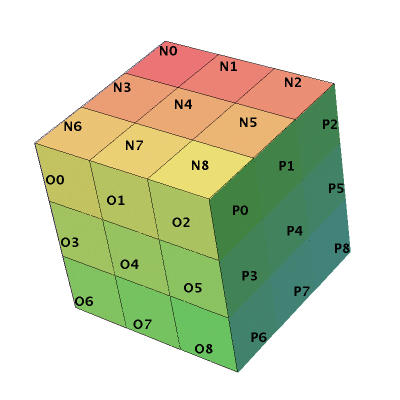
\includegraphics[scale=0.47]{fig-children_grid1_00_cube.png} \\}

\caption{(a) An $\nside = 3$, resolution $i$, rHEALPix planar cell with ID $s$ showing its $\nside^2 = 9$ resolution $i + 1$ subcells labelled with their IDs. Their row and column numbers are highlighted in red.
(b) The cell adjacency structure of $G_1$ for the (0, 0)-rHEALPix map projection with $\nside = 3$.}
\end{figure}

The proposed OGC DGGS Standard specifies that cell identifiers must uniquely identify cells across all resolutions, and that cell IDs are defined with an addressing method that uses at least one of hierarchy, space filling curve, coordinate or encoded address. The cell identifiers described here are unique with both hierarchical and space filling properties.

%-----------------------------------------------------------------------------
\section{Cell identifiers and their topological relationships}\label{sec:cellgeom}
The proposed OGC DGGS Standard proposes that DGGS should support the DE-9IM topological relationships. The cell IDs described above have a number of properties that allow us to compute both cell adjacency and DE-9IM topological relationships very efficiently directly from the cell ID without recourse to latitude longitude coordinates. Adjacency is computed by considering each numeric digit as a $base_3$ tuple whose two digits are the row and column numbers within the parent - highlighted in red in figure~\ref{fig:children}(a). The cell IDs of adjacent cells at any chosen resolution can be found using $base_3$ fraction maths on rows and columns. Just as in $base_1_0$ maths to add 0.010 to a $base_1_0$ fraction, we only need to add 1 to the second digit past the decimal point, so we can use an equivalent construct in $base_3$ for row and column maths at any resolution by simply operating on the digit representing the desired resolution.

The cell adjacency structure of the ellipsoidal hierarchy $G'$ induces a cell adjacency structure on the planar hierarchy $G$ that can be visualized by folding $G_0$ into a cube along its cell edges, and this is how the rHEALPix DGGS can be construed as a geodesic DGGS; see figure~\ref{fig:children}(b). The row and column neighbours of $O2$ are $N8$, $P0$, $O5$, and $O1$. We need a mechanism to traverse cells from face to face as well as within faces. To accomplish this we treat faces as integers and assigned them the following ($row_3$, $column_4$) integer pairs N($0_3,0_4$), O($1_3,0_4$) P($1_3,1_4$), Q($1_3,2_4$), R($1_3,3_4$), S($2_3,0_4$). With this arrangement $base_3$ maths will result in the correct north-south face transitions between the N--O, and O--S face pairs. Similarly $base_4$ maths on the column integers will ensure correct east-west  transitions between the equatorial face pairs of O--P, P--Q, Q--R and R--O. While it may seem strange to mix bases within the same number, these are strings not numbers so we can treat each digit the way we need to.

Returning to our initial example $O2$ in row,column notation is ($1_3.0_3,0_4.2_3$). Traversing from $O2$ to $O1$ is achieved by subtracting $.1_3$ from $O2$'s column and from $O2$ to $O5$ by adding $.1_3$ to $O2$'s row. i.e. ($1_3.0_3,0_4.2_3-.1_3$) evaluates to ($1_3.0_3,0_4.1_3$) = $O1$ and ($1_3.0_3+.1_3,0_4.2_3$) evaluates to ($1_3.1_3,0_4.2_3$) = $O5$. Similarly adding $.1_3$ to $O2$'s column we get  ($1_3.0_3,0_4.2_3+.1_3$) which evaluates to ($1_3.0_3,1_4.0_3$) = $P0$ and subtracting $.1_3$ from $O2$'s row we get ($1_3.0_3-.1_3,0_4.2_3$) which evaluates to ($0_3.2_3,0_4.2_3$) = $N8$.

Traversing between faces N or S and P, Q or R requires an additional step to account for the different geometries of the planar vs ellipsoidal grids. This is most simply achieved by constructing a translation logic table from invalid ID's that are generated by the above maths to valid ones. Without giving the complete solution, note in figure~\ref{fig:children}(b) that  $P0$, $P1$ and $P2$ have as their neighbours $N8$, $N5$ and $N2$ respectively. It turns out that at the junction of the N and P faces the pattern $0,1,2$ recursively translates to the pattern $8,5,2$ at every resolution so this logic can be readily coded. Similarly recurring patterns occur for the other N or S and P, Q or R transitions.

To compute DE-9IM topological relationships between cells we will often compare two IDs to determine if their most significant digits starting with $(N | O | \cdots | S)$ match, and then examine the properties of the rightmost digits that differ. We will refer to the sequence of matching digits as $\IDparent$ and the two strings of remaining digits as each cell's $\IDchild$. For cells $O234546$ and $O234787$ their $\IDparent$ is $O234$ and their $\IDchild$ are $546$ and $787$ respectively.

We will also need to define three types of cell neighbour:

\begin{enumerate}[(i)]
    \item A cell's row-neighbours are the set of cells at the same resolution, who's rows are the same and columns differ by 1. To account for transitions between the N or S and P, Q or R faces 'differ by 1' is used in this and the next two as shorthand to include the additional translational step required to traverse between the faces,
    \item A cell's column-neighbours are the set of cells at the same resolution, who's columns are the same and rows differ by 1,
    \item A cell's diagonal-neighbours are the set of cells at the same resolution, who's rows and columns differ by 1, 
\end{enumerate}
 
The DE-9IM topological relationships are usually referred to by the operators: equals, within, contains, touches, disjoint, covers, coveredBy, intersects, crosses and overlaps. 

The following list demonstrates how each of these relationships can be determined by manipulating cell IDs using the constructs we have described above.

\begin{enumerate}[(i)]
    \item Cell $A$ and cell $B$ are equal if they have an $\IDparent$ and both $A$ and $B$'s $\IDchild$ strings are null,
    \item If cell $A$ and cell $B$ share an $\IDparent$ and $B$'s $\IDchild$ string is null then $A$ is within $B$ and $B$ contains $A$, 
    \item If cell $A$ is within cell $B$ then $A$ touches $B$ on a edge if  $A$'s $\IDchild$ string satisfies $(0 | 1 | 2)^* | (2 | 5 | 8)^* | (0 | 3 | 6)^* | (6 | 7 | 8)^*$. $A$ touches $B$ on a corner (ie two edges) if $A$'s $\IDchild$ string satisfies $( 0 )^* | (2 )^* | ( 6 )^* | ( 8 )^*$. For example $O234787$ touches $O234$ on an edge and $O234666$ touches $O234$ on a corner.
    \item If length $A$ is greater than length $B$ and $A$ NOT within cell $B$ then $A$ touches $B$ on an edge if at least one of $A$'s row- or column- neighbours is within $B$.   $A$ touches $B$ on a point if one $A$'s diagonal-neighbours is within $B$,
    \item Cell $A$ and cell $B$ are disjoint if ($A$ NOT equal $B$) AND ($A$ NOT within $B$) AND ($A$ NOT contain $B$) AND ($A$ NOT touches $B$),
    \item $A$ covers $B$ only if $A$ contains $B$, and $A$ is coveredBy $B$ only if $A$ is within $B$,
    \item We note that because of the way cells are defined, no single cell can intersect, cross, or overlap another cell.
\end{enumerate}

Irregular shapes may be represented geometrically by lists of cell IDs, and any level of precision can be represented by including cells of appropriately small size. It follows that the above tests may be extended to two irregular shapes by extending the above comparisons to comparisons of the members in two ID's lists, each representing one of the two irregular shapes. While this can be inefficient in a traditional serial processing environment, it is ideally suited to modern parallel processing environments.

%-----------------------------------------------------------------------------
\section{Conclusion}
We have revisited the original definition of the rHEALPix DGGS and identified those geometric and cell identifier properties that make it conformant with the  new Discrete Global Grid System Core Standard being proposed by the Open Geospatial Consortium. We have also demonstrated that rHEALPix DGGS cell IDs can be used directly to efficiently compute each of the DE-9IM topological relationships, which have emerged as a part of the proposed standard, but weren't explicitly part of earlier work on DGGS. This comparison of the proposed standard with an existing DGGS is a useful first step in showing how the standard can be applied.

%-----------------------------------------------------------------------------
%\section*{References}
\bibliographystyle{iopart-num}
\bibliography{DE2015_S3A-3_GibbR_The-rHEALPix_DGGS}

\ack
This research was funded through Landcare Research's Core Funding contract with the New Zealand government science funding agency, the Ministry of Business, Innovation and Employment. 

\end{document}

